\documentclass[11pt,a4paper]{ivoa}
\input tthdefs

\newcommand{\xtype}[1]{\texttt{#1}}

\usepackage{listings}
\lstloadlanguages{XML,sh}
\lstset{flexiblecolumns=true,basicstyle=\small,tagstyle=\ttfamily}
\usepackage[utf8]{inputenc}
\usepackage{todonotes}
\usepackage{textcomp}
\usepackage{float}
\usepackage{lscape}
\usepackage{longtable}
\hyphenation{image/mosaic}

\title{IVOA Obscore Extension for Radio data}

\ivoagroup{Data Model Working Group}

\author{Fran\c cois Bonnarel}
\author{Mireille Louys}
\author{Baptiste Cecconi}
\author{Vincenzo Galluzzi}
\author{Yan Grange}
\author{Mark Kettenis}
\author{Mark Lacy}
\author{Alan Loh}
\author{Mattia Mancini}
\author{Peter Teuben}
\author{Alessandra Zanichelli}



\editor{Fran\c cois Bonnarel}

\previousversion{}

       


\begin{document}

\begin{abstract}
This is a proposed extension to the Obscore specification for description of radio data.
\end{abstract}

\section*{Acknowledgments}

The authors would like to thank all the participants in DM-WG and Radioastronomy-IG discussions 
for their ideas, critical reviews, and contributions to this document.
We acknowledge also the support of  ESCAPE (European Science Cluster of Astronomy
and Particle Physics ESFRI Research Infrastructures) funded by the EU Horizon
2020 research and innovation program (Grant Agreement no 824064).
% are there other grants from partners to mention here?

\section{Introduction}


ObsCore specification \citep{2017ivoa.spec.0509L} defines both a minimal datamodel to describe datasets 
and a table consistent with the model which can be served by TAP services. It has been successful 
to define a lot of data discovery services in astronomy.

The emergence  of  the Radioastronomy Interest Group in the IVOA in April 2020 confirmed the strong 
interest of the radio astronomy community to distribute their data in the VO. Many teams now 
distribute their data using VO standards\footnote{https://ivoa.net/documents/Notes/RadioVOImp/index.html}. 
While reduced radio data products, such as images or spectral cubes, %(and single dish data - {\it is that true ?} ) 
are mostly covered by the ObsCore model, the lower level observational data 
(interferometric visibilities, single dish data in SDFITS, filterbank or whatever other specific formats) require additional description parameters. For interferometry, this was already exposed 
in 2010 when Anita Richards wrote a note called "Radio interferometry data in the VO" 
\footnote{https://wiki.ivoa.net/internal/IVOA/SiaInterface/Anita-InterferometryVO.pdf} which is 
still worth reading. Among other goals, the current specification tries to cover the needs exposed in this note. See appendix \ref{ADQLusecases} for more normalized user scenarii in term of ADQL queries.
% Mireille an attempt to widen the scope ??
With the expansion of large radio astronomy projects such as LOFAR, NenuFAR, the future SKA, ngVLA, etc...
and the emergence of interesting research topics matching data in all electromagnetic regimes, the 
Virtual Observatory framework can facilitate a wider access to radio data for experts and 
non-specialists radio astronomers in order to support collaborations in multi-wavelength, 
multi-messenger astronomy. 

%mireille:
% the needs for today as explored in recent meetings in Escape framework can also be summarized here
% add a short paragraph here
%Although the interferometry data are nowadays dominant in radio field, similar issues occur for 
%optical interferometry data. The extension we are defining here is valid for both domains.  


\begin{figure}[H]
\centering

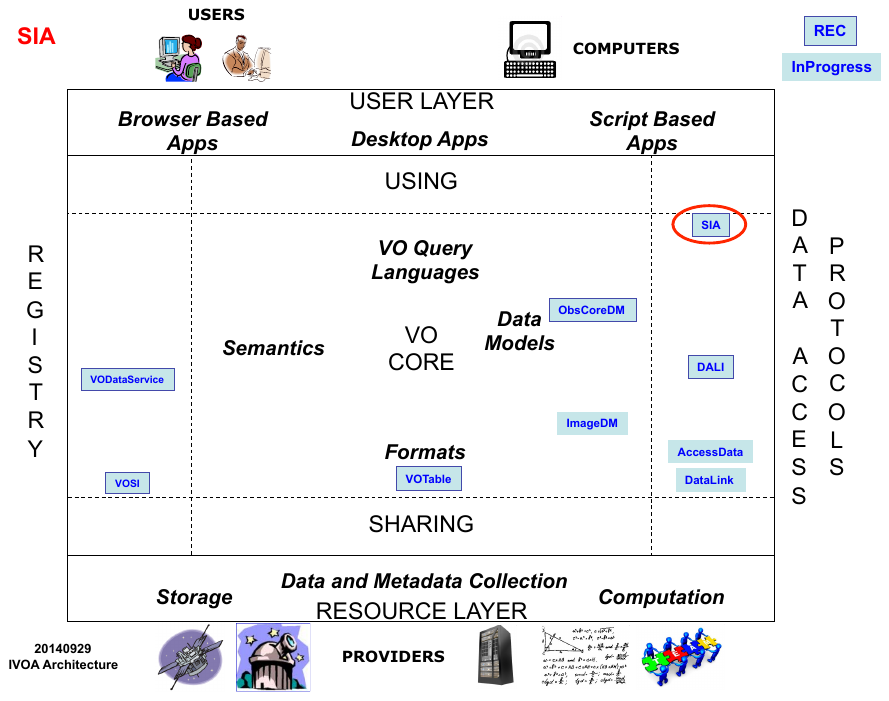
\includegraphics[width=0.9\textwidth]{archdiag.png}
\label{fig:architecture}
\end{figure}

% Mireille : it seems this is not the good diagram but the one of SIA 
% change architexture diag

%The role of this Visibility ObsCore extension in the IVOA is very close to ObsCore itself. It's only a fine grain improvement of this specification. 
% Mireille's  suggestion 
The scope of this Radio ObsCore extension in the IVOA is very close to ObsCore itself. 
Its goal is to add new specific features to the existing ObsCore metadata tables and expose 
them in the ObsTAP TAP\_SCHEMA. 





\section{Radio data specifities from the Data Discovery point of view}
\label{sec:specificities}

On the lower end of the radio spectrum, radio astronomers generally make use of 
frequencies for designating the spectral ranges of their observation. The standard 
ObsCore attributes em\_min em\_max  are in wavelength and are not really convenient. 
That's why we should also provide their translation into frequencies. 
        
Receivers with a (ultra)wide bandwidth, up to tens of GHz, are 
nowadays commonly used for both interferometric and Single Dish (herefater SD) radio observations. 
Given that the spatial field of view and resolution linearly depend on wavelength, these quantities may significantly vary across the observed bandwidth in a radio observation. 
Generally only a representative value (for instance the median) for these two parameters can be given. It is 
noticeable that this is the case for any measuring system allowing a large interval of 
$\lambda/D$ (where $\lambda$ and $D$ are the wavelengths and the measuring system
aperture scale).
 
Similarly, the resolution power quantity, commonly provided to describe optical spectroscopic data, does not make much sense in the radio domain and it is generally not used.
To properly represent radio data it would be necessary to introduce a new ObsCore term for the absolute spectral resolution in frequency unit, for which a representative value for each observation can be given. 

%We note that the interpretation of the spatial field of view as based on a mid/representative value for $\lambda$ should be better clarified in the ObsCore definition of this parameter.
%We also point out that in the radio domain the field of view is an instantaneous concept, i.e. the instantaneous footprint (a circular primary beam in the case of mono-feed receivers, a more complex shape in the case of multi-feed/beamforming/PAFs), while in ObsCore it is defined as the approximate size of the region covered by the data product. 
%This means that the region covered by an observation can be larger than the instantaneous field of view. This happens for instance in a SD radio map, in an interferometric map/mosaic, etc.

Modern radio instrumentation offer the possibility of {\it n} different spectral windows within the same observation with significant separation or different resolutions.
Such observations may be represented at the highest granularity as many entries in an ObsCore Table. However it's up to data provider to decide which level of granularity is best adapted in order to optimize data discoverability and ease data access, depending on the scientific content of the observation (see Sect. \ref{subsec:sd} for an example).

%Modern radio instrumentation offer the possibility of {\it n} different spectral windows within the same observation. 
%If the more common approach to ObsCore is applied, such observations would be represented at the highest granularity as many entries in an ObsCore Table. However, this might puzzle a user trying to understand the actual setup of the observation. In order to optimize data discoverability and ease data access, different levels of granularity may be adopted depending on the scientific content of the observation (see Sect. \ref{subsec:sd} for an example).

%The introduction of sky\_scan\_mode in ObsCore Extension is useful to describe the spatial scanning strategies in both interferomentric and SD radio observations. However, its definition does not encompass scan modes in the spectral domain, like frequency switching or spectral scan. A more general scan\_mode term would better represent both the spatial and the spectral scanning modes. Alternatively, a further parameter frequency\_scan\_mode for the spectral domain aloce could be added in the ObsCore Extension for radio data.



\subsection{Single dish data}\label{subsec:sd}

Single Dish observations can be done with different types of receiving systems. Typical frontends are mono-feed, multi-feed and phased array feed (PAF), the last two suitable to efficiently span wider parts of the sky. 
Data can be acquired by various backend systems providing either the total intensity (integrated over the whole available bandwidth) or the spectroscopic/spectropolarimetric intensity (acquired in each spectral channel/sample).
Data are saved as raw counts resulting from the digitisation of the voltage signal measured by the receiving system.
Commonly-used SD data formats are registered FITS standard conventions (FITS, SDFITS and MBFITS) or unregistered conventions like the standard FITS-based format delivered by the INAF radio telescopes.

The combination of telescope, frontend and backend permits the realization of various observing strategies characterized by specific spatial and/or spectral patterns.
Typical SD observing strategies are: on source, frequency switching, ON-OFF observations, raster or on-the-fly (OTF) mapping, raster or OTF cross-scan, skydip calibrations, see Fig~\ref{fig:SD}. For each spatial position in the observation, SD data gather emission for any of the spectral samples in the given frequency band and polarization.  
If multi-feed/PAFs are used, a set of spatial positions are simultaneously measured. Scan modes should be described in ObsCore in order to allow astronomers to better understand the structure of the data which will be retrieved.

Spatial resolution in the SD case is intended as the beam size. This holds true for any type of receivers, since also for multi-feed/PAF ones the spatial resolution is ruled by the size of the individual beam. 

Contrary to what usually happens for  interferometric observations, for some radio telescopes a SD observation (scan) contains only one scientific target (for example INAF ones). In any case, each target in an observation is listed as a separate entry in an ObsCore Table sharing the same obs\_id.

Complex frequency setups are possible in the same observation, as already mentioned in Sect. \ref{sec:specificities}.
%For instance, new multi-band receivers acquire simultaneously different frequency bands with different setups (bandwidth, max/min frequency, etc.). Moreover, modern digital backends allow the simultaneous acquisition of more than one spectral window (each with its spectral resolution) inside each receiver band. Such a complex observation should be properly represented in an ObsCore Table.
%As an example: the new tri-band K-Q-W receiver being installed on board of the INAF radio telescopes observes simultaneously the K, Q and W frequency bands in the same observations. It can be coupled with a digital backend delivering {\it n} different spectral windows for each of the three observed bands. In this example, if the highest-granularity approach to ObsCore is applied, such a case would be described with $3n$ entries in a ``flat'' ObsCore Table. In case of broadband spectro-polarimetric observations, like the simultaneous study of many emission lines, $n$ may become large. Thus, such numerous ObsCore entries associated to the same dataset might make it difficult for a user to understand the observing setup. The possibility to adopt different levels of granularity in an ObsCore Table might be considered.

The ObsCore definition of t\_resolution as the minimal interpretable interval between two points along the
time axis (being it an average or representative value) is generally not applicable for SD data. Typically time is not an independent variable in SD measurements, it can be saved together with spatial/spectral/intensity information as a timestamp associated to each data sample.
Even in the case of on-source tracking, time information in SD data is not intended for time domain studies.

%Finally, also in the SD case we note that currently allowed terms for dataproduct\_type do not permit a proper data characterisation. A revision of the reserved list of terms for dataproduct\_type is currently under discussion within IVOA.





\begin{figure}[H]
\centering

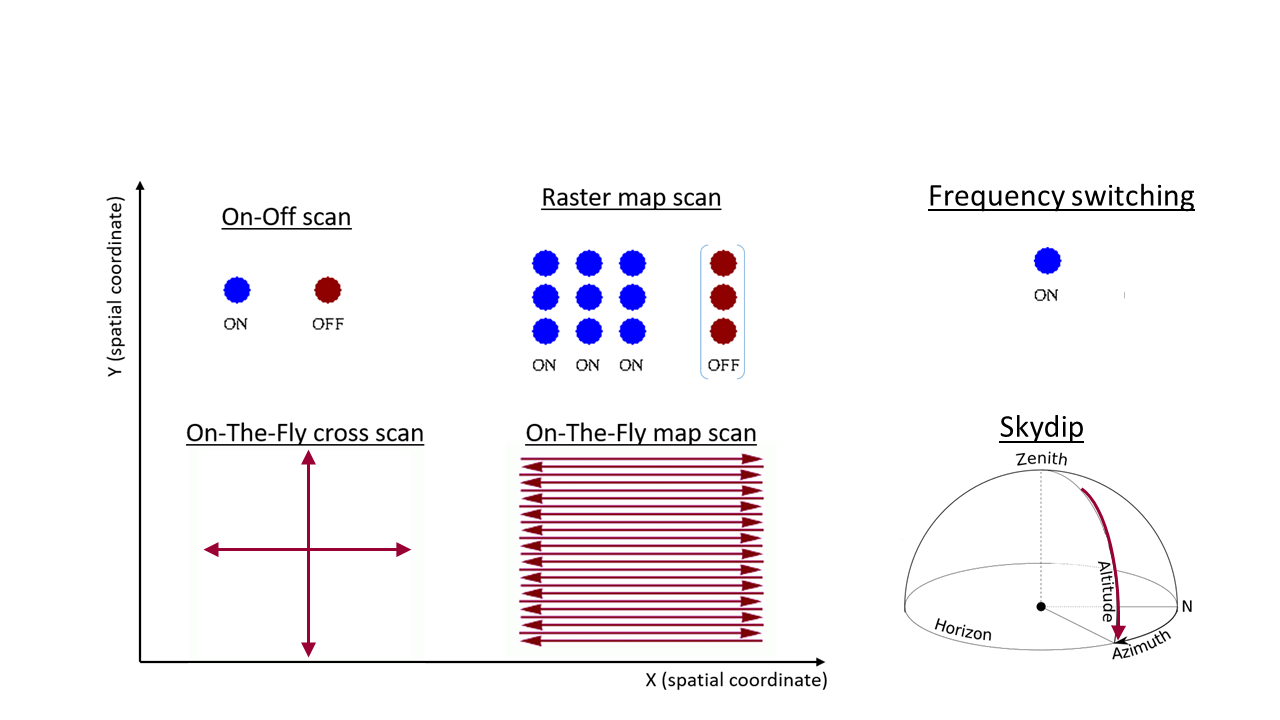
\includegraphics[width=0.9\textwidth]{SingleDish.png}
\caption{Single Dish Observation scan modes}
\label{fig:SD}
\end{figure}



\subsection{Visibility data }
\label{sec:visibility}

Visibility data are sets of complex numbers corresponding to the amplitude and phase 
of correlation coefficients measured between pair of antennas (i.e., a baseline), at 
a given time, a given wavelength or polarisation. The visibility data are a sparse 
representation of the observed sky. The visibility data sets can be processed to obtain 
interferometric images, through inverse Fourier algorithms. Each visibility measurement 
corresponds to an interferometric fringe system on the sky. 

The imaging algorithms include a calibration step allowing to set the center of the 
reconstructed image, setting this direction as a phase reference. The visibilities
are then usually represented in a spatial frequency plane, called the \emph{uv} plane, 
whose orientation is perpendicular to phase reference direction. The instantaneous PSF 
(Point Spread Function) of an interferometer is the Fourier transform of all baselines 
sampled in the \emph{uv} plane. Hence, the quality of the reconstructed images are 
directly related to the set of baselines used for the measurements.

Visibility data are usually organised as sets of matrices for various phase references
(i.e., pointing, or fields) and configuration of the baselines, such as their
distances and orientations. Such matrices may or may not be regularly sampled in time, 
wavelength and polarisation.
    
%How can the ObsCore parameters describe the characterization of these observations? 
As for any other observation product described with ObsCore, the description may be split into
several records in the ObsCore table, when ObsCore parameters cannot represent the 
variety of the observation results coverage (e.g., if there are several observed ``fields'', 
requiring different s\_ra and s\_dec value, or various groups of spectral bands, etc.) 

We consider that consistent ObsCore records as described above defines datasets with 
a dataproduct type set to ``visibility''.


Contrary to what occurs with direct imaging observations, the PSF of the interferometer
is filtering spatial scales (large scales, when the small baselines are insufficiently 
sampled; and vice versa for small scales with long baselines).
For large spectral ranges, the variations of the field of view and the spatial resolution 
along the axis may become so large that the typical value cannot be sufficient to 
characterize the dataset. Ranges of values for such parameters are required to accurately 
describe such datasets.

The quality of the data strongly depends from the distribution of the visibility measurements 
in the uv plane : the more complete the uv sampling plane, the better the reconstructed image. 
The uv plane distribution can be characterized by several numbers. 
The minimal and maximum distance between measurements in the uv plane provide assessments for 
spatial resolution and largest angular scale. 
Beside this a uv plane filling factor of the distribution will allow to predict the quality 
of reconstruction of the image in the distance plane (sky).
Eventually, the ellipticity of the distribution is a measure of the distortions that can 
affect the reconstruction.

Radioastronomers also check the quality of the visibility data by looking at some maps of 
the data structure. The uv coverage map can show how complete and regular is the sampling in 
the \emph{uv} plane and give an hint of resolution and maximum angular scale. 
The visualisation of the dirty beam, which is the Fourier transform of the \emph{uv} sampling 
function gives an hint of the intrinsic quality of possible reconstruction. As maps they are 
not queriable. So links to these kind of maps will not be exposed in the extension 
table but only via a DataLink service. 

If none of these \emph{uv} characterization features are available to be exposed in the service 
we can still predict ranges of some of those by using some kind of facility description.  
Important features are the antenna diameter (or maximum antenna diameter), the number of 
antennas and the minimum and maximum distance between antennas of the array.

In addition to these specifities most of the scan modes shown on figure~\ref{fig:SD} also 
apply to some interferometry observations and should be described. 

\section{ObsCore attributes definition valid for radio data}
\label{sec:ObsCoreRadDef}

%Some mandatory or optional parameters will have peculiar estimation for visibility data.
For radio data some of the definitions on Obscore datamodel elements need to be adjusted 
to fit the peculiarity of medata for datasets partition, uv space, etc.

\subsection{obs\_id}

Astronomers usually know what they identify as a single observation : a complex set of 
measurements made in a given sequence of time. obs\_id should define unambiguously each 
observation.

\subsection{obs\_publisher\_did}

Radio data observations can be split in several subparts with homogeneous spatial, 
time, spectral coverage intervals, spectral resolution, etc. Each part can be described by 
a single ObsCore dataset and has its own obs\_publisher\_did. It has to be unique in the 
Virtual Observatory domain.

\subsection{s\_fov}
\label{sec:fov}

A typical value for the field of view size is to be computed on the observation by taking into account the sky scan geometry and receiver type in use.
s\_fov coincides with the instantaneous field of view $\lambda / D$ only for pointed observations (for instance, an ON in the SD case) obtained with a mono-feed receiver. In this case, $\lambda$ is the mid value of the spectral range and D coincides with the telescope diameter (SD case) or the largest diameter of the array antennae or telescopes (interferometric case). 



\subsection{s\_resolution}
\label{sec:res}
In the case of single dish using mono- or multi-feed/PAF receivers this is the beam size inferred from the wavelength and telescope diameter. 
In the case of interferometry, a typical value for the spatial resolution will be given by $\lambda / L$ where $\lambda$ 
is the mid value of the spectral range and L is the typical longest distance in the \emph{uv} plane.
For beamforming applied to SD s\_resolution is set by the size of one individual electronically-formed beam, while in the interferometric case it is ruled by the maximum distance among the stations.
 
 
\subsection{s\_region}
For single dish data it will strongly depend on the scanning mode and type of receiver in use.
This shape will be the typical contour of the detectable beam for interferometry. Of course it cannot be accurate. 

\subsection{o\_ucd}

In the current UCD vocabulary (UCD1+ controlled vocabulary - Updated List of Terms Version 1.5) there appear to be no primary words suitable to describe raw SD data. o\_ucd=phot.flux.density, which fits well for appropriate data, does not seem appropriate, since the single dish measured quantity is expressed in raw counts coming from the digitisation of a voltage signal generated in the receiver chain by the incoming electromagnetic field. Further discussion on o\_ucd is ongoing within the Semantics WG.

In the case of visibility data the "observable" is a complex number representing Fourier 
coefficients of the image Fourier transform. Its UCD string is \emph{stat.fourier}. 

\subsection{t\_exptime}
Total duration of the observation for the given dataset/ObsCore entry. Example: in case of multiple targets, t\_exptime will be computed for each source and written in the appropriate ObsCore Table entry. 


\subsection{t\_resolution}
Not applicable for single dish data (see Sect. \ref{subsec:sd}). For interferometric observations it is the integration time set at the correlation level.

\subsection{dataproduct\_type and dataproduct\_subtype}

Radio astronomy data cover a wide variety of dataproduct\_types from visibility for raw interferometry data to cubes, images, spectra, time series or even measurements (in the case of single dish on scan mode). Single dish observations in some modes show specifities which are not covered by the current ObsCore dataproduct\_type vocabulary. This is the case of spatial profiles obtained with on the fly cross scan or of the tables of flux measurements obtained on a regular spatial grid but with specific time stamp for each spot as in the raster map  mode.
A new external standard IVOA vocabulary is currently defined for dataproduct types\footnote{https://www.ivoa.net/rdf/product-type/2023-06-26/product-type.html} an tackles some of these specificities
However some of them SHOULD be covered in the dataproduct\_subtype attribute if no new term is introduced in the standard vocabulary.

\section{ObsCore extension for radio data}

Table \ref{tab:ExtensionAtt} shows the %additional 
parameters we propose to add to ObsCore in order to better describe radio single dish and visibility data.
The last column indicates if the attribute is useful for all radio datasets or only for visibilities, beamforming, or single dish data.
Two options have be considered in the TAP or SIA services descriptions: 
\begin{itemize}
\item adding the new data model elements directly into the main ObsCore table
\item providing an extra table for these, named ivoa.visibilities for instance,  which will 
be joined to the main table. 
\end{itemize}
This specification is based on the first option, but with some suggestion ti implement also the second one as stated in section \ref{sec:implementation}

\subsection{spatial parameters}
s\_fov\_min, s\_fov\_max are estimated like the typical value (see subsection \ref{sec:fov}). 
In the case of SD pointed observations with mono-feed receivers and the majority of interferometric observations the minimum and maximum $\lambda$ values in the spectral range(s) will be used in the formula. In the case of mapping scans or multi-feed/PAF receivers s\_fov\_min and s\_fov\_max are derived as the minimum and maximum sizes of the circular region encompassing the covered area.

s\_resolution\_min, s\_resolution\_max are estimated like the typical value (see subsection \ref{sec:res}) where $\lambda$ is replaced by the minimum and maximum wavelength of the spectral range(s). The size D is the telescope diameter for SD observations and the largest distance in the uv plane. Beamforming may represent an exception to this rule, see \ref{sec:res}.

In the case of interferometry, the s\_maximum\_angular\_scale is estimated as $\lambda/l$ where $\lambda$ is the typical 
wavelength and l is the typical smallest distance in the uv plane. 

\subsection{frequency characterization}

As was stated above (\ref{sec:specificities}) radioastronomers use frequency quantities to characterize their datasets. Therefore we introduce three additional parameters in the extension : f\_min and f\_max for spectral ranges and f\_resolution for absolute spectral resolution .

\textit{To avoid inconsistensies between the core attributes em\_min, em\_max and em\_respower and these additional quantities we suggest to compute these new quantities when building a view on top of the basic ObsCore table. The frequency attributes MUST be expressed in khz to allow interoperability.} 
\subsection{uv parameters}
These parameters are valid for interferometry only.

%uv\_distance\_min and uv\_distance\_max are straigthforward.
The absolute uv\_distance\_min and uv\_distance\_max  in the uv plane give some outlier minimum and maximum scale in some direction.
%are evaluated by fitting an ellipse on the visibilities present in the uv plane.

% Mireille but still for the spec it is good to redefine them here
To compute the ellipse's eccentricity of the UV distribution a principal component analysis 
(PCA) with 2 components is performed over the data points sampling the UV plane to select the 
main axis of data scattering. 
The first component is used to rotate the distribution of UV in a way that the major variation 
of the distribution is leaning towards the $x$ axis of a bi dimensional $xy$ Cartesian plane. 
The major axis length and the minor axis length of the ellipse are therefore defined as the 
semi distance between the most positive point along the $x$/$y$ axis and the most negative point 
among the $y$ axis. For instance, if the range of the rotated UV will cover on the $x \in [-10, 
10]$ the major axis distance would be 10, a similar procedure is done on the y axis. This 
procedure allows the definition of the \emph{UV} distribution eccentricity:

uv\_distribution\_exc computed as follows:
\begin{equation}
uv\_distribution\_exc = \sqrt{1-\frac{b^2}{a^2}}
\end{equation}
where a is the major axis length and b is the minor axis length.
The filling factor of the UV plane (hereafter uv\_distribution\_fill) is computed as the average 
number of samples found in a $N^{uv}_{samples}$x$N^{uv}_{samples}$ equi-spaced grid enclosing the 
rotated ellipse. In formulas, the boundaries of a cell (i,j) are defined by the boundaries
\begin{equation}
u \in [u_{min} + \frac{u_{max} - u_{min}}{N^{uv}_{samples}} \cdot i , u_{min} + \frac{u_{max} - 
u_{min}}{N^{uv}_{samples}} \cdot (i + 1)]
\end{equation} 
and
\begin{equation}
v \in [v_{min} + \frac{v_{max} - v_{min}}{N^{uv}_{samples}} \cdot j , v_{min} + \frac{v_{max} - 
v_{min}}{N^{uv}_{samples}} \cdot (j + 1)]
\end{equation} 
where $u_{max}$/$v_{max}$ are the respective maximum u/v of the \emph{uv} sample and 
$u_{min}$/$v_{min}$ is the minimum u/v of the \emph{uv} sample.

Given the above boundaries the number of samples within a cell (i,j) will be $n^{uv}_{i,j}$ 
and uv\_distribution\_fill will be then computed as 
\begin{equation}
uv\_distribution\_fill = \frac{\sum^{N^{uv}_{samples}}_{i=1} \sum^{N^{uv}_{samples}}_{j=1} 
n^{uv}_{i,j} }{(N^{uv}_{samples}) ^ 2},
\end{equation}

in the preliminary analysis $N^{uv}_{samples} = 1000$.


% Mireille: moved time param below uv space because uv plane deals with spatial features 

\subsection{time parameters}
t\_exp\_min, t\_exp\_max and t\_exp\_mean are added in the case of variation in the individual timestamps 
duration. This is usually not the case for SD data and these parameters will be set to NULL.


\subsection{Observation modes and instrumental parameters}
These parameters are intended to describe the main telescope(s) characteristics for both SD antennas and interferometers. Such instrumental characteristics give an approximate idea on the spanned angular scales, field of view, product types, etc.

The more global parameter to define is the instrument type allowing to discriminate single dish observations from interferometry or beam forming. 

Parameters instrument\_ant\_number, instrument\_ant\_min\_dist and instrument\_ant\_max\_dist are related to interferometers only while instrument\_ant\_diameter, instrument\_feed are valid also for SD.
We note that instrument\_feed could also  account for the number of beams in the case of a beamforming/PAF receiver.

The scanning strategy adopted in an observation is described by the parameter scan\_mode. This parameter covers both spatial and frequency scanning modes (see Sect.~\ref{subsec:sd} for details). 
Scanning parameters are applicable to both SD and interferometry.

Pointing mode distinguishes targeted observations from  fixed alt-azimuth or wobble ones. The ObsLocTAP specification \citep{2021ivoa.spec.0724S} defines the term tracking\_type for describing this as well as a  vocabulary for these modes. We include the same term as an extension parameter here.


\subsection{Auxiliary datasets useful for data quality estimation}

Auxiliary datasets such as  uv distribution map, dirty beam maps, frequency/amplitude plots, phase/amplitude plots are useful for astronomers to check data quality.  
In that case DataLink \citep{2015ivoa.spec.0617D} may provide a solution to attach these auxliary data to ObsCore records. The semantics FIELD in the \{link\} response  will contain \#auxiliary  for links to these maps or plots while  the content\_qualifier FIELD introduced from 1.1  could contain a vocabulary as defined in this ObsCore extension in table \ref{tab:ExtensionAtt}.


\section{How to implement the extension in a TAP service}i
\label{sec:implementation}

The ObsCore extension for radio (including or not visibility data) described above SHOULD  be added to the main ObsCore table. The standardID for this extented table will be ivo://ivoa.net/std/ObsCore\#radioExt-1.0". This implies that the the core ObsCore attributes follow version 1.1 of the Obscore standard.
\textit{ In practice a  table containing only the extension attributes  MAY be added to the same schema. The full extension table will then be a view joining the core table and the  table with extension attribue only via an extended ObsTAP ADQL query. A single dataset in each observation will be associated to a single row in ObsCore. It will be identified by a unique obs\_publisher\_did. This obs\_publisher\_did can be used as a foreign key to join the main table and the extension table.}

In the registry, the Obscore table and the Extended table MUST be described in the tableset of the service. They will show respectively the ObsCore Model utype "ivo://ivoa.net/std/ObsCore\#core-1.0" an the extended Obscore Model utype "ivo://ivoa.net/std/ObsCore\#radioExt-1.0" . 




        
\begin{landscape}
\begin{longtable}{l  p{4cm} p{4cm} p{4.5cm} l l l}
\sptablerule
\textbf{column name}&\textbf{definition}&\textbf{utype}&\textbf{ucd}&\textbf{unit}&\textbf{validity}\cr
\sptablerule
\sptablerule
\texttt{ s\_resolution\_min}&\texttt{ Angular resolution, longest baseline and  max frequency dependant}&{ Char.SpatialAxis.\newline Resolution.Bounds.\newline Limits.LoLim}&{pos.angResolution;stat.min}&{arcsec}&radio\cr
\sptablerule
\texttt{s\_resolution\_max}&\texttt{Angular resolution, longest baseline and min frequency dependant}&\texttt{Char.SpatialAxis.\newline Resolution.Bounds.\newline Limits.HiLim}&{pos.angResolution;stat.max}&arcsec&radio\cr
\sptablerule
\texttt{s\_fov\_min}&\texttt{field of view diameter,  min value, max frequency dependant}&\texttt{Char.SpatialAxis.\newline Coverage.Bounds.\newline Extent.LowLim}&{phys.angSize;instr.fov;\newline stat.min}&deg&radio\cr
\sptablerule
\texttt{s\_fov\_max}&\texttt{field of view diameter,  max value, min frequency dependant}&\texttt{Char.SpatialAxis.\newline Coverage.Bounds.\newline Extent.HiLim}&{phys.angSize;instr.fov;\newline stat.max}&deg&radio\cr
\sptablerule
\texttt{s\_maximum\_angular\_scale}&\texttt{maximum scale in dataset, shortest baseline and  frequency dependant}&\texttt{Char.SpatialAxis.\newline Resolution.Scale.\newline Limits.HiLim}&{phys.angSize;stat.max}&arcsec&interferometry\cr
\sptablerule
\texttt{f\_min}&\texttt{spectral coverage min in frequency}&\texttt{Char.SpectralAxis.\newline Coverage.Bounds\newline Limits.LoLim}&{em.freq;stat.min}&Mhz&radio\cr
\sptablerule
\texttt{f\_max}&\texttt{spectral coverage max in frequency}&\texttt{Char.SpectralAxis.\newline Coverage.Bounds\newline Limits.HiLim}&{em.freq;stat.max}&Mhz&radio\cr
\sptablerule
\texttt{f\_rsolution}&\texttt{absolute spectral resolution in frequency}&\texttt{Char.SpectralAxis.\newline Coverage.Bounds\newline Limits.HiLim}&{em.freq;stat.max}&Khz&radio\cr
\sptablerule
\texttt{t\_exp\_min}&\texttt{minimum integration time per sample}&\texttt{Char.TimeAxis.\newline Sampling.Extent\newline LoLim}&{time.duration;obs.exposure;\newline stat.min}&s&radio\cr
\sptablerule
\texttt{t\_exp\_max}&\texttt{maximum integration time per sample}&\texttt{Char.TimeAxis.\newline Sampling.Extent\newline HiLim}&{time.duration;obs.exposure;\newline stat.max}&s&radio\cr
\sptablerule
\texttt{t\_exp\_mean}&\texttt{average integration time per sample}&\texttt{Char.TimeAxis.\newline Sampling.Extent\newline HiLim}&{time.duration;obs.exposure\newline stat.mean}&s&radio\cr
\sptablerule
\texttt{uv\_distance\_min}&\texttt{minimal distance in uv plane}&\texttt{Char.UVAxis.\newline  Coverage.Bounds.\newline Limits.LoLim}&stat.fourier;pos;stat.min&m&interferometry \cr
\sptablerule
\texttt{uv\_distance\_max}&\texttt{maximal distance in uv plane}&\texttt{Char.UVAxis.\newline  Coverage.Bounds.\newline Limits.LoLim}&stat.fourier;pos;stat.max&m&interferometry \cr
\sptablerule
\texttt{uv\_distribution\_ecc}&\texttt{eccentricity of uv distribution}&\texttt{Char.UVAxis.\newline  Coverage.Bounds.\newline Eccentricity}&stat.fourier;pos&&interferometry \cr
\sptablerule
\texttt{uv\_distribution\_fill}&\texttt{filling factor of uv distribution}&\texttt{Char.UVAxis.\newline  Coverage.Bounds.\newline FillingFactor}&stat.fourier;pos;arith.ratio&&interferometry \cr
\sptablerule
% mireille here for antennas features , it is clear it belongs to instrument. 
%Not useful to use the term in the name .
%\texttt{instrument\_ant\_number}&\texttt{number of antennas in array}&\texttt{Provenance.ObsConfig.\newline Instrument.Array.\newline AntNumber}&instr.baseline;meta.number& \cr
%\sptablerule
\texttt{instrument\_ant\_number}&\texttt{number of antennas in array}&\texttt{Provenance.ObsConfig.\newline Instrument.Array.\newline AntNumber}&meta.number;instr.param&&interferometry, beamforming \cr
\sptablerule
% same for all antenae features
\texttt{instrument\_ant\_min\_dist}&\texttt{minimum distance between antennas in array}&\texttt{Provenance.ObsConfig.\newline Instrument.Array.\newline MinDist}&instr.baseline;stat.min&m&interferometry \cr
\sptablerule
\texttt{instrument\_ant\_max\_dist}&\texttt{maximum distance between antennas in array}&\texttt{Provenance.ObsConfig.\newline Instrument.Array.\newline MaxDist}&instr.baseline;stat.max&m&interferometry \cr
\sptablerule
\texttt{instrument\_ant\_diameter}&\texttt{diameter of telecope or antennas in array}&\texttt{Provenance.ObsConfig.\newline Instrument.Array.\newline Diameter}&instr.param&m&radio \cr
\sptablerule
\texttt{instrument\_feed}&\texttt{number of feeds}&\texttt{Provenance.ObsConfig.\newline Instrument.Feed}&instr.param&& radio  \cr
\sptablerule
\texttt{scan\_mode}&\texttt{scan mode (on-off, \newline raster map, on-the-fly map,...)\newline }&\texttt{Provenance.\newline Observation.\newline sky\_scan\_mode}&instr.param&& radio \cr
\sptablerule
\texttt{tracking\_mode}&\texttt{targeted, alt-azimuth, wobble, ...)\newline }&\texttt{Provenance.\newline Observation.\newline tracking\_mode}&instr.param&& radio \cr
\sptablerule
\texttt{uv\_distribution\_map}&\texttt{uv distribution map}&\texttt{Char.UVAxis.\newline  Sampling.\newline Sensitivity.Map}&stat.fourier;pos;meta.ref.url&&interferometry \cr
\sptablerule
\texttt{s\_beam\_dirty}&\texttt{dirty beam}&\texttt{- (via DataLink}&{via DataLink}&&interferometry\cr
\sptablerule
\texttt{phase\_amplitude}&\texttt{phase amplitude plot}&\texttt{via DataLink}&{via DataLink}&&interferometry\cr
\sptablerule
\texttt{frequency\_amplitude}&\texttt{dirty beam}&\texttt{via DataLink}&{via DataLink}&&interferometry\cr
\sptablerule
\caption{ObsCore radio data extension parameters proposal}
\label{tab:ExtensionAtt}
\end{longtable}
\end{landscape}

\appendix

\section{Science use cases and translation to ADQL queries  based on ObsCore Radio extension  }
\label{ADQLusecases}

\subsection{Science case }
\subsection{Use case - s\_resolution\_min}
\textit{Comparative study of low surface brightness extended emission surrounding compact sources, like for instance Virgo A. Select any dataset map (raster or on-the-fly) with s\_resolution\_min larger than the desired spatial resolution of 1 arcmin.}
Show me all datasets satisfying: \\
I. Minimum spatial resolution < 0.017 deg \\
II Target Virgo A or position inside 15 arcmin from 187.7059308,+12.3911232 \\
III Scan mode is raster map or on-the-fly map

\begin{verbatim}
s_resolution_min > 0.017 AND
WHERE (target_name = 'Virgo A' OR
CONTAINS(POINT(s_ra, s_dec),CIRCLE,187.7059308,+12.3911232,0.25)) = 1)) AND
(scan_mode = 'raster map' OR scan_mode = 'on-the-fly map')
\end{verbatim}

\subsection{Use case - s\_resolution\_max}
\textit{Morphological study of SNR IC443. Select any dataset of type map (raster or on-the-fly) with s\_resolution\_max less than the desired spatial resolution of 1 arcmin.}

Show me all datasets satisfying: \\
I. Maximum spatial resolution < 0.017 deg \\
II Target IC443 or position inside 15 arcmin from 94.2500000,+22.5699997 \\

\begin{verbatim}
s_resolution_max < 0.017 AND
WHERE (target_name = 'IC443' OR
CONTAINS(POINT(s_ra,s_dec),CIRCLE(94.2500000,+22.5699997,0.25)) = 1)) AND
(scan_mode = 'raster map' OR scan_mode = 'on-the-fly map')
\end{verbatim}

\subsection{Use case - s\_fov\_min A}
\textit{Select any dataset with minimum field of view larger than 0.8 degree. For instance, investigate the region surrounding cluster Abell 194.}

Show me all datasets satisfying:\\
I. Minimum FOV > 0.8 deg \\
II Target name = Abell 194 or position inside 15 arcmin from 21.5054167, -1.3672221 \\
\begin{verbatim}
SELECT * FROM ivoa.ObscoreRadioExtended
WHERE s_fov_min > 0.8 AND
(target_name = 'Abell 194' OR
CONTAINS(POINT(s_ra,s_dec),CIRCLE(21.5054167,-1.3672221,0.25)) = 1)) AND
(scan_mode = 'raster map' OR scan_mode = 'on-the-fly map')
\end{verbatim}

\subsection{Use case - s\_fov\_min B}
\textit{Pictor A has a typical angular extension  arcminutes , select any image/cube completely containing the target}
Show me all datasets satisfying: \\
I. Target name = Pictor A \\
II. The circle defined by the minimum FOV of the dataset fully contains the circle delimiting Pictor A. \\
\begin{verbatim}
WHERE target_name = 'Pictor A' AND
CONTAINS(CIRCLE(79.9571789, -45.7788479,(8/60)/2),
CIRCLE(s_ra, s_dec, s_fov_min/2)) = 1)
\end{verbatim}

Nb: The above queries can be run with s\_resolution\_min and s\_fov\_max instead of s\_resolution\_max and s\_fov\_min respectively, to obtain results in which at least part of the dataset satisfy the condition.
For instance, consider datasets with a large observed bandwidth, like those taken with wide/ultrawide band receivers.
The condition s\_resolution\_max<d\_typical may not be satisfied. At the same time, the user may want to select those dataset where the desired condition on spatial resolution is matched at least partially  within the observed band.

\subsection{Use case - dataproduct\_type}
\textit{Select all observations of calibrator source 3C48 with the Medicina Grueff radio telescope at frequencies in the range 20-21 GHz, to investigate its flux variability (light curve) in the years 2000-2023}
Show me all datasets satisfying: \\
I. Target name = 3C 48 \\
II. obs\_collection = ?INAF-Medicina, single dish?\\
III. Observed frequency in the range 20-21 GHz \\
IV. dataproduct\_type = spatial\_profile or dataproduct\_type = map\\
V. 51544 < observation time (MJD) < 60309 \\
\begin{verbatim}
SELECT * FROM ivoa.ObscoreRadioExtended
WHERE obs_collection EQ ?INAF-Medicina, single dish? AND
(em_min >=20000 AND em_max <= 21000) AND
(dataproduct_type EQ 'spatial profile' OR scan_mode LIKE "*map*") AND
target_name = '3C48' AND
(t_min >= 51544 AND t_max <= 60309)
\end{verbatim}

\subsection{Use case - f\_resolution, f\_min, f\_max}
\textit{Select any cube with spectral resolution better than 1 MHz and spectral range inside the 1 to 1.5 GHz band.}

Show me all datasets satisfying:\\
I. Product type is cube \\
II. spectral resolution better than 1 MHz \\
f\_min and f\_max are computed by means of a user defined function. \\
\begin{verbatim}
SELECT * FROM ivoa.ObscoreRadioExtended
WHERE dataproduct_type = 'cube' AND
f_resolution < 1000000 AND
f_min > 1.0 e+9 AND
f_max < 1.5e+9
\end{verbatim}

% Mireille Louys: shall we also look for spectra with these frequency constrains ? 


 
% end section Alexandra's science case 

\subsection{FB : Use case 1.1 data product and targer object selection }
\textit{Any raw interferometry observation containing target Fornax cluster.}\\
\\
Show me all  observation identifiers satisfying:\\
I. DataType = visibility \\
II. Target Name = Fornax Cluster \\
\begin{verbatim}
      SELECT obs_id FROM ivoa.ObscoreRadioExtended
      WHERE dataproduct_type = 'visibility'
      target_name = 'Fornax cluster'
\end{verbatim}
\subsection{Use case 1.2}
\textit{Any  dataset with minimum field of view larger than 0.5 degree.}\\
\\
Show me all datasets satisfying:\\
I. Minimum FOV > 0.5 deg \\
\begin{verbatim}
      SELECT * FROM ivoa.ObscoreRadioExtended
      WHERE fov_min > 0.5 
\end{verbatim}

\subsection{Use case 1.3/ time selection }
\textit{Any cube  with absolute spectral resolution better than 1 Mhz and spectral range inside the 1 to 1.5 Ghz band.}\\ \\
Show me all datasets satisfying:\\
I. Product type is cube \\
II. spectral resolution better than 1Mhz \\
III. lower spectral limit > 1Ghz \\
IV. higher spectral limit < 1.5Ghz 
\begin{verbatim}
      SELECT * FROM ivoa.ObscoreRadioExtended
      WHERE dataproduct_type = 'cube' AND
      f_resolution < 1000 AND
      f_min > 1000 AND
      f_max < 1500
\end{verbatim} 

\subsection{Use case 1.4 / freq selection }
\textit{Any low frequency image or cube  defined as smaller than 1 Ghz.}\\ \\
Show me all datasets satisfying:\\
I. Product type is image or cube \\
II. higher spectral limit < 1Ghz
\begin{verbatim}
      SELECT * FROM ivoa.ObscoreRadioExtended
      WHERE (dataproduct_type = 'image' OR
      dataproduct_type = 'cube') AND
      f_max  < 1000
\end{verbatim}

\subsection{Use case 1.5 / scale selection}
\textit{Any visibility dataset  where  maximum angular scale is larger than 0.5degrees.}\\ \\
Show me all datasets satisfying:\\
I. Product type is visibility \\
II. Maximum angular scale  >  0.5 deg 
\begin{verbatim}
      SELECT * FROM ivoa.ObscoreRadioExtended
      WHERE dataproduct_type = 'visibility' AND
      max_angular_scale > 0.5 
\end{verbatim}

\subsection{Use case 1.6 / instrument type and mode selection }
\textit{Any single dish  dataset  in raster mode around 3C 273.}\\ \\
Show me all datasets satisfying:\\
I. Instrument type is Single dish \\
II. Scan mode is raster \\
III. Target name = 3C 273 or \\
IV. position inside 3 arcmin around  	187.2779159404900 +02.0523882305500
\begin{verbatim}
      SELECT * FROM ivoa.ObscoreRadioExtended
      WHERE instrument_type = 'SD' AND
      scan_mode = 'raster' AND
      (target_name = '3C 273' OR
       CONTAINS(POINT(s_ra,s_dec), CIRCLE(187.2779159404900, +02.0523882305500,0.05)) = 1)     
\end{verbatim}

% use case FB 
\subsection{Use case 1.7 instrument type selection}
\textit{Any single dish or beam forming dataset  with spectral range inside the 500 Mhz - 1Ghz band and in the Coma Cluster.}\\ \\
Show me all datasets satisfying:\\
I. Instrument type is Single dish or beam forming \\
II. lower spectral limit > 500 Mhz \\
III. higher spectral limit < 1Ghz \\
IV. position inside 18 arcmin around 194.93502 +27.91246
\begin{verbatim}
      SELECT * FROM ivoa.ObscoreRadioExtended
      WHERE (instrument_type = 'SD' OR
      instrument_type = 'beamForming') AND
      CONTAINS(POINT(s_ra,s_dec),CIRCLE(194.93502, +27.91246, 0.3) = 1     
\end{verbatim}


\subsection{Use case 1.8 instrument type and freq selection }
\textit{Any single dish or beam forming dataset  with spectral range inside the 500 Mhz - 1Ghz band and in the Coma Cluster.}\\ \\
Show me all datasets satisfying:\\
I. Instrument type is Single dish or beam forming \\
II. lower spectral limit > 500 Mhz \\
III. higher spectral limit < 1Ghz \\
IV. position inside 18 arcmin around 194.93502 +27.91246

\begin{verbatim}
      SELECT * FROM ivoa.ObscoreRadioExtended
      WHERE (instrument_type = 'SD' OR
      instrument_type = 'beamForming') AND
      f_min > 500 AND
      f_max < 1000 AND
      CONTAINS(POINT(s_ra,s_dec),CIRCLE(194.93502, +27.91246, 0.3) = 1     
\end{verbatim}


\subsection{Use case 1.9 uv distribution selection}
\textit{Any visibility data of good quality from th uv distribution point of view.}\\ \\
Show me all datasets satisfying:\\
I. Product type = visibility \\
II. uv distribution filling factor  > 0.7 \\
III. uv distribtion factor eccentricity  < 0.1 \\

\begin{verbatim}
      SELECT * FROM ivoa.ObscoreRadioExtended
      WHERE dataproduct_type = 'visibilty' AND
      uv_distribution_fill > 0.7 AND
      uv_distribution_ecc < 0.1  
\end{verbatim}


\subsection{Use case 1.10 -instrument parameters selection }
\textit{Any interferometry data of good quality and significant spatial resolution from the instrumental point of view. }\\ \\
Show me all datasets satisfying:\\
I. Instrument type = visibility \\
II. number of antennae > 40 \\
III. antenna maximum distance in meters  > 5000 \\

\begin{verbatim}
      SELECT * FROM ivoa.ObscoreRadioExtended
      WHERE instrument_type = 'interferometry' AND
      instrument_ant_number > 40 AND
      instrument_ant_max_dist > 5000 
\end{verbatim}


\subsection{Use case 1.11 - time selection }
\textit{Any timeseries obtained in beam forming mode with time resolution better than 0.1 second and time sample maximal duration smaller than 0.05 second. }\\ \\
Show me all datasets satisfying:\\
I. Instrument type = beam forming\\
II. Product type = time series  \\
III. time resolution < 0.1 s\\
IIV. maximal duration per sample  < 0.05 s \\

\begin{verbatim}
      SELECT * FROM ivoa.ObscoreRadioExtended
      WHERE instrument_type = 'beamForming' AND
      dataproduct_type = 'timeseries' AND
      t_resolution < 0.1 AND
      t_exp_max < 0.05 
\end{verbatim}



\bibliography{ivoatex/ivoabib,ivoatex/docrepo}

\end{document}
